\documentclass[a4paper, 11pt]{article}
\usepackage{graphicx}
\usepackage{booktabs}
\usepackage{hyperref}
\usepackage{listings}
\usepackage{microtype}
\usepackage[utf8]{inputenc}
\usepackage[ngerman]{babel}
%\usepackage{fullpage} % changes the margin

\graphicspath{{img/}}

\lstdefinestyle{mystyle}{
    basicstyle=\footnotesize,
    breakatwhitespace=false,         
    breaklines=true,  
    frame = single,               
    captionpos=b,                    
    keepspaces=true,                 
    numbers=left,                    
    numbersep=5pt,                  
    showspaces=false,                
    showstringspaces=false,
    showtabs=false,                  
    tabsize=2
}
\lstset{style=mystyle}

\begin{document}
\noindent
\large\textbf{Arduino: Secure Fridge} \hfill \textbf{SoSe'18} \\
\normalsize Hardwarenahe Systemprogrammierung \hfill Leonard Koll, 1133123 \\
Prof. Dr. Peter Sturm \hfill Paul Kugener, 1071658

\section{Projektbeschreibung}
Das Ziel der Veranstaltung war die Einarbeitung in hardwarenahe Systeme sowie deren Planung und Programmierung. Als begleitendes Praxisprojekt wurde ein Sicherheitssystem für die Überwachung von Kühlschränken im Bürobereich entwickelt. Bei öffentlichen Kühlschränken, welche von vielen Personen genutzt werden, ist oft nicht klar einsehbar, wer den Kühlschrank nutzt und welche Produkte entnommen werden.

Das entwickelte Sicherheitssystem protokolliert mit Hilfe einer Kamera die Nutzung des Kühlschranks. Bei jeder Öffnung des Kühlschrankes wird der Nutzer durch ein RFID-Token identifiziert. Die Token-ID und das aufgenommene Foto werden auf einer Micro-SD gespeichert.

Das folgende Kapitel beschreibt die Einzelkomponenten des Projektes. Danach wird der Systemaufbau dargestellt und der Funktionsablauf des Systems näher erläutert. Anschließend wird eine eigene Kommunikationslibrary vorgestellt, welche spezifisch auf dieses Projekt zugeschnitten wurde.


\section{Komponenten}
\begin{description}
\item [Microcontroller-Board] Der \textit{Arduino Uno}, basierend auf dem Atmega328 Chip, stellt das Herzstück des Projekts dar. Im Arduino wird der Kontrollfluss des ganzen Systems bestimmt. Alle weiteren Sensoren (Komponenten) werden an den Arduino angeschlossen und deren Daten werden im Arduino verarbeitet.
\item [Kamera] Als Kamera wurde die \textit{Adafruit TTL JPEG Camera (VC0706 chipset)} benutzt. Die Kamera zeichnet sich vor allem durch ihre Bedienbarkeit und die umfangreiche Bibliothek aus. So kann beispielsweise durch eine simple Setter-Methode die Auflösung der Fotos festgelegt werden (640x480, 320x240 oder 160x120). Auch liegt der aktuelle Schnappschuss des Kamera-Moduls als komprimierte JPEG-Datei im Buffer vor und kann so in speichergerechten Teilen vom Arduino eingelesen werden.
\item [Nutzeridentifizierung] Zur Nutzererkennung wird ein \textit{MFRC522 RFID Reader} verwendet. Das Modul ermöglicht das Lesen der Informationen eines RFID-Tokens durch elektromagnetische Wellen. Unterschiedliche RFID-Token repräsentieren in unserem Projekt die verschiedenen Mitarbeiter. Durch die Token-Überprüfung kann festgestellt werden, ob dem Nutzer die Nutzung des Kühlschrank erlaubt war oder nicht. 
\item [Speichermedium] Die erfassten Daten können durch ein \textit{Micro-SD-Card Modul} auf einer Micro-SD-Karte abgespeichert werden. Die Daten setzen sich zusammen aus dem Bildmaterial, welches von der Kamera gelesen wird und den Informationen der Nutzer, welche durch das RFID Modul erfasst werden.
\item [Button] Das Öffnen der Kühlschranktür wird durch das Drücken eines Buttons simuliert. Das Signal des Buttons dient als Trigger für einen Protokollierungsauftrag.
\end{description}


\section{Systemaufbau}
\begin{figure}[htb]
\centering
    {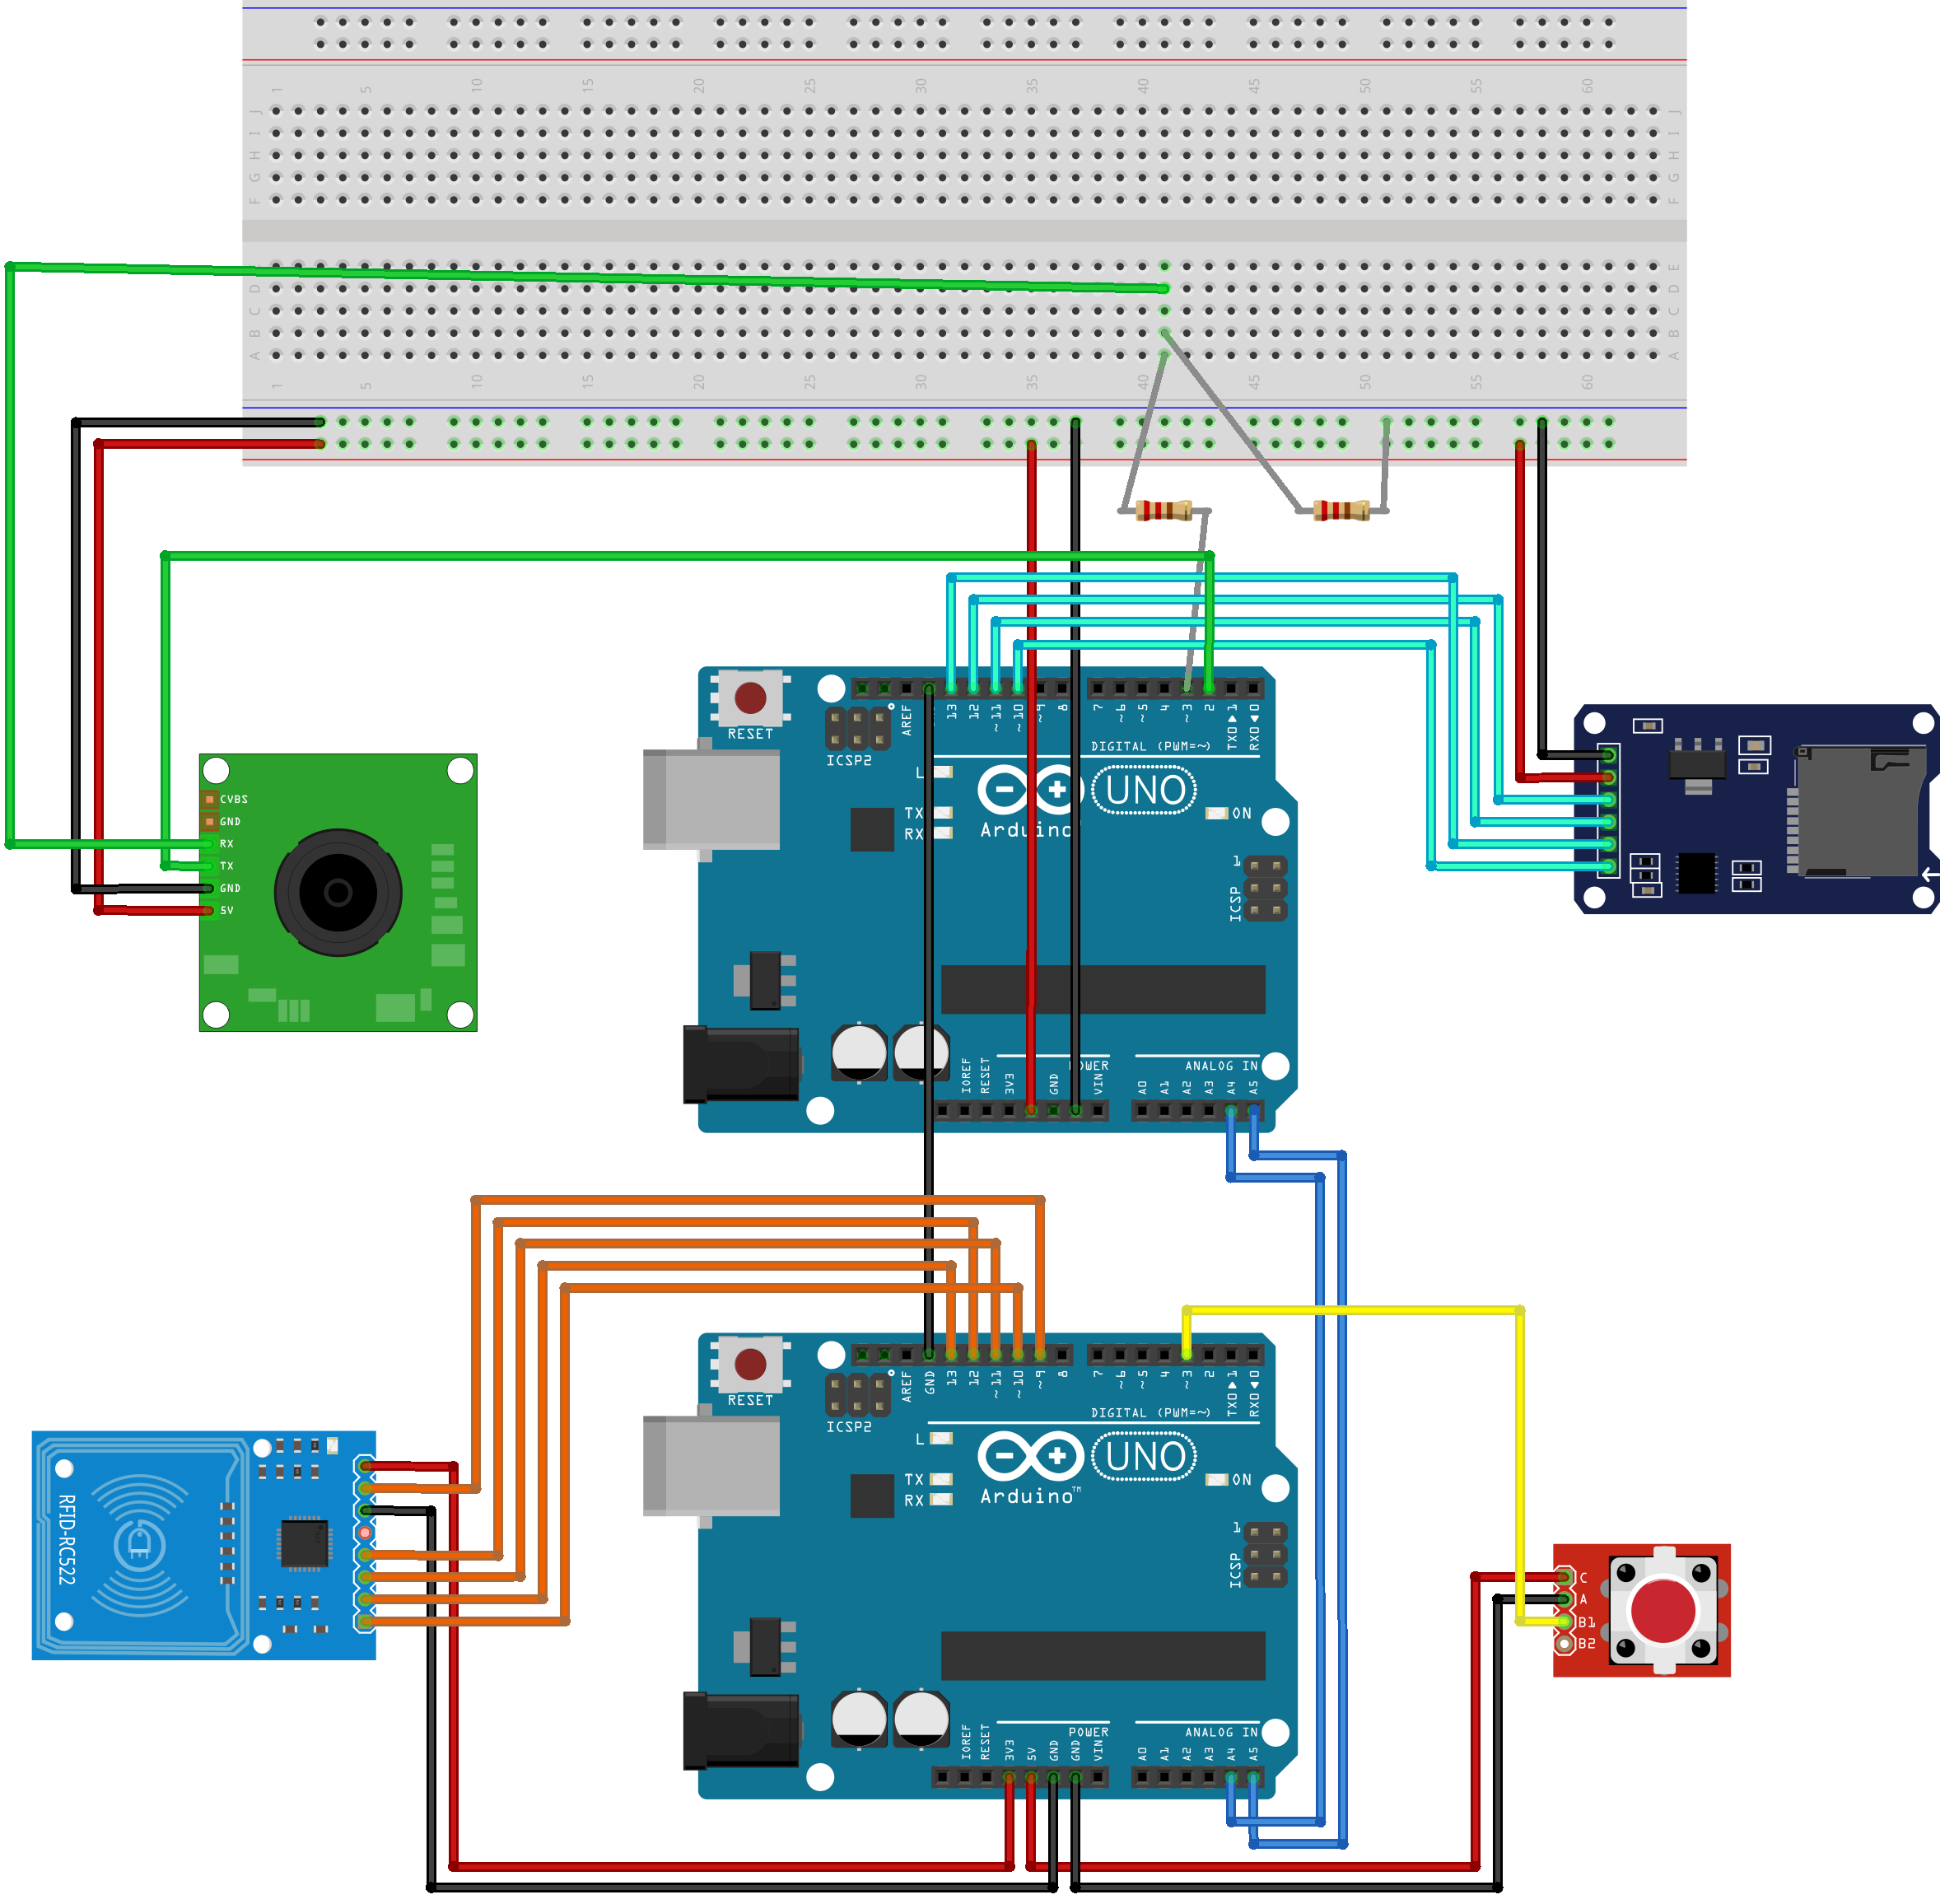
\includegraphics[width=1\textwidth]{uebersicht.png}}
    \caption{Verbindung der Komponenten in Steckplattenansicht\label{fig:uebersicht}}
\centering
\end{figure}

\noindent Der Aufbau des Überwachungssystems lässt sich in zwei Teilsysteme eingliedern. Beide Teilsysteme bestehen, wie in Abbildung \ref{fig:uebersicht} zu erkennen ist, aus jeweils einem \textit{Arduino Uno} und zwei weiteren Komponenten. 

Als erstes Teilsystem kann das in der Abbildung untere System betrachtet werden. Die verbundenen Komponenten sind der Button und das RFID-Modul.
Das zweite Teilsystem beinhaltet die Kamera und das SD-Karten-Modul. In der Abbildung ist zu erkennen, dass zwischen dem \texttt{RX}-Pin der Kamera und dem Arduino zwei \textit{Resistoren} geschaltet sind.

Die Kommunikation zwischen den beiden Teilsystemen läuft über zwei Verbindungen von analogen Arduino-Pins. Die Untergliederung des Systems in zwei Komponenten ermöglicht eine räumlich getrennte Anbringung von Identifikationseinheit und Kamera. Die Schnittstellenanbindungen der Komponenten ist in der nachfolgenden Tabelle ablesbar.


\begin{table}[htb]
\begin{tabular}{@{}lllll@{}}
\toprule
\multicolumn{2}{c}{Arduino 1} &  & \multicolumn{2}{c}{Arduino 2}                    \\ \cmidrule(r){1-2} \cmidrule(l){4-5} 
RFID\_SDA    & arduino\_d10   &  & CAMERA\_TX  & arduino\_d2                        \\
RFID\_SCK    & arduino\_d13   &  & CAMERA\_RX  & resistor $\rightarrow$ GND         \\
RFID\_MOSI   & arduino\_d11   &  &             & resistor $\rightarrow$ arduino\_d3 \\
RFID\_MISO   & arduino\_d12   &  & CAMERA\_GND & GND                                \\
RFID\_IRQ    & not connected  &  & CAMERA\_VCC & 5V                                 \\
RFID\_RST    & arduino\_d9    &  &             &                                    \\ 
RFID\_GND    & GND            &  & SD\_CS      & arduino\_d10                       \\
RFID\_VCC    & 3.3V           &  & SD\_SCK     & arduino\_d13                       \\
                &                &  & SD\_MOSI    & arduino\_d11                       \\
BTN\_S       & arduino\_d3    &  & SD\_MISO    & arduino\_d12                       \\
BTN\_-       & GND            &  & SD\_GND     & GND                                \\
BTN\_+       & 5V             &  & SD\_VCC     & 5V                                 \\ \bottomrule
\end{tabular}
\end{table}


\section{Funktionsablauf}
Der Funktionsablauf des Sicherheitssystems wurde im Sequenzdiagramm in Abbildung \ref{fig:sequenz} dargestellt.

Ein Protokollierungsauftrag startet mit dem Öffnen der Kühlschranktür, was durch das Drücken des Buttons simuliert wird. Das System ermittelt daraufhin unter Zurhilfenahme des RFID-Moduls die Identität des Nutzers. Wird ein Token erkannt, wird kontrolliert, ob diesem Nutzer der Zugriff zum Kühlschrank gestattet ist. Anhand dieser Informationen wird nun ein \texttt{Request-String} gebildet und an den zweiten Arduino übertragen. Dieser String beinhaltet mehrere Informationen:
%\pagebreak
\begin{enumerate}
\item Wurde ein Nutzer-Token benutzt?
\item Ist der Nutzer berechtigt, den Kühlschrank zu benutzen?
\item Nutzer-ID
\end{enumerate}

\noindent Das Eintreffen des \texttt{Request-String} löst beim zweiten Arduino ein \textit{Event} aus, welches die Aufnahme eines Fotos sowie dessen Speicherung auf der Miro-SD Karte triggert. Zusätzlich wird in einem Text-Log hinterlegt, welcher \texttt{Request-String} mit welcher Foto-Datei assoziiert ist. Dies beendet einen Protokollierungsauftrag. Das Analysieren der Kühlschranknutzung kann folglich durch die Betrachtung der Logs und den Vergleich mit dem Bildmaterial durchgeführt werden. 

\begin{figure}[htb]
\centering
    {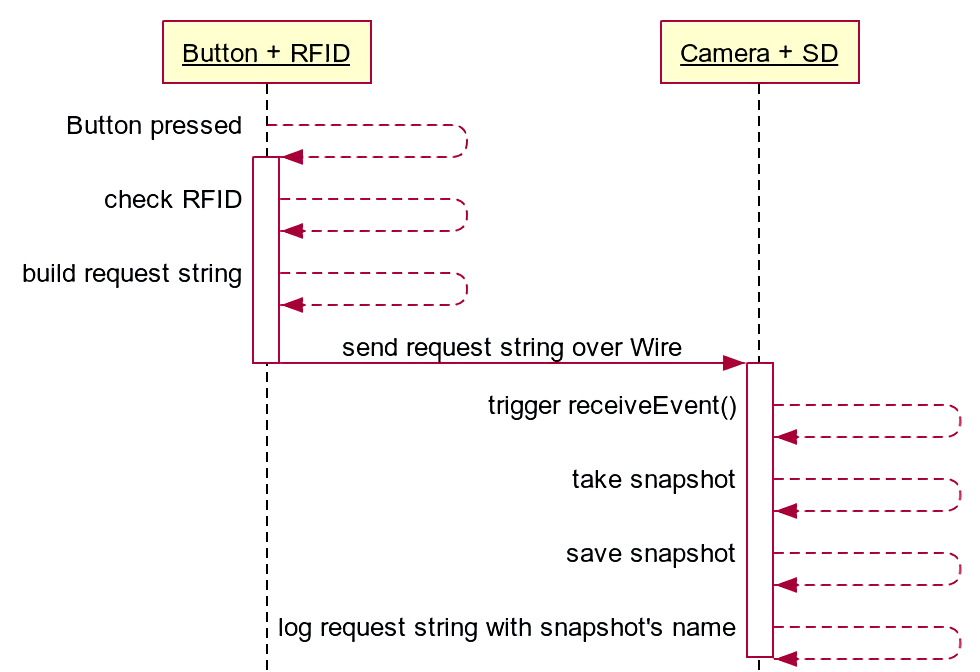
\includegraphics[width=.9\textwidth]{sequenz1.png}}
    \caption{Funktionsablauf anhand eines Sequenzdiagramms\label{fig:sequenz}}
\centering
\end{figure}


\section{Eigene Library zur Kommunikation}
\begin{figure}[htb]
    \centering
        {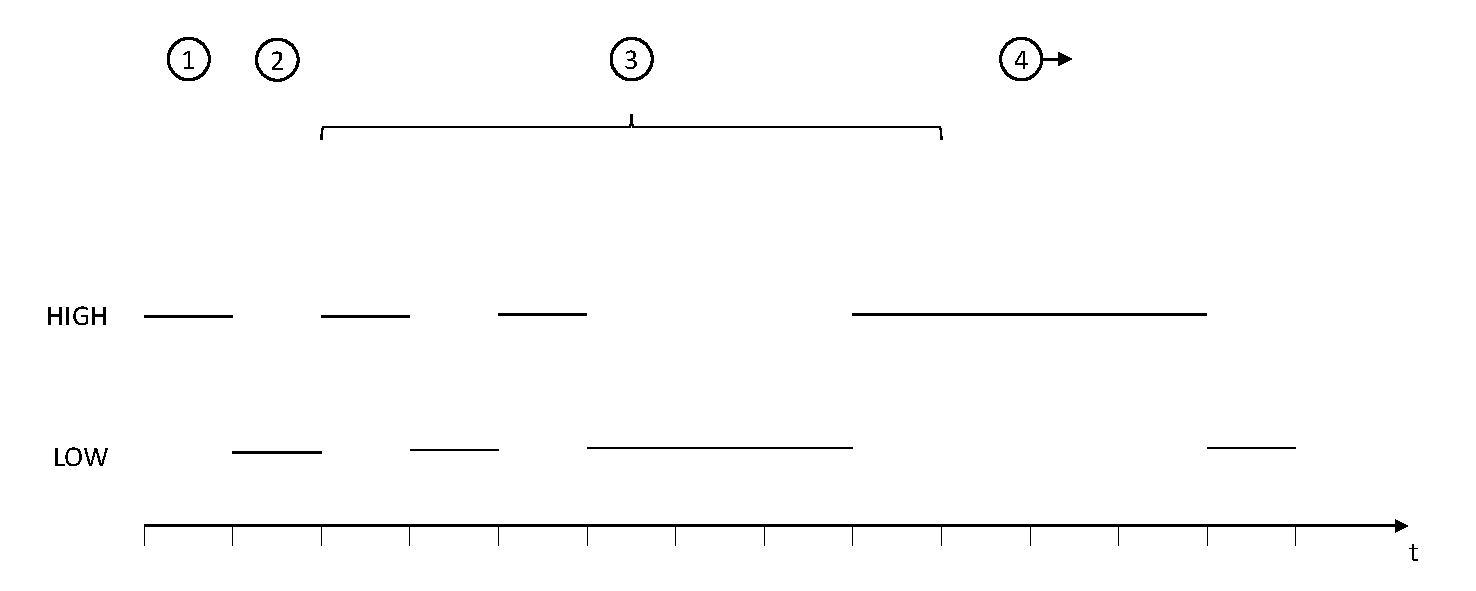
\includegraphics[width=1\textwidth]{signal.pdf}}
        \caption{Ablaufschema Signalübertragung \label{fig:signal}}
    \centering
\end{figure}
Abbildung \ref{fig:uebersicht} zeigt die ursprüngliche Konfiguration des Projektes, in welcher die Kommunikation zwischen den Arduinos über die Wire-Bibliothek (I2C) und die Ports \texttt{A4} (data line / Datenübertragung) und \texttt{A5} (clock line / Synchronisation) abgewickelt wurde. Motivation für eine eigene Implementierung war der Wunsch, in einem Teilbereich des Projektes auf den Komfort und die Abstraktion einer heruntergeladenen Bibliothek zu verzichten. Geplant war außerdem der Einsatz eines 433 Mhz Sender/Receiver Paares anstelle einer Kabelverbindung, wesshalb das Protokoll ein Heartbeatsignal enthält.

Die entwickelte Bibliothek sieht die Verwendung von nur einem Kabel über einen jeweils frei wählbaren Digitalpin vor. Abbildung \ref{fig:signal} visualisiert die Impulse während einer Datenübertragung. Da es sich um ein binäres Signal handelt, wird nur zwischen \texttt{HIGH} und \texttt{LOW} unterschieden. Auf der x-Achse ist die Zeit aufgetragen. In der vorliegenden Konfiguration der Library entspricht eine Zeiteinheit 2ms. Werden keine Daten übertragen, so ist die Leitungs spannungsfrei (\texttt{LOW}). Sobald Kommunikationsbedarf besteht, wird ein \texttt{HIGH}-Implus versendet (1). Dieser Impuls dient zugleich zur zeitlichen Synchronisation von Sender und Empfänger. Der zweite Implus fungiert als Heartbeat-Indikator. Ist er \texttt{HIGH}, so handelt es sich um ein Heartbeat-Signal und es sind keine weiteren Signale zu erwarten. Ist er \texttt{LOW}, so wechselt der Empfänger in den Datenempfangsmodus. Die Abschnitte (3,4) zeigen die Anfänge einer Datenübertragung; Das Byte in Abschnitt (3) beschreibt exemplarisch die ASCII-Codierung eines "Q". \newline

\noindent\begin{minipage}{\textwidth}
    \lstinputlisting [caption=Verwendung der Connector Library, label=libuse]{img/code.txt}
\end{minipage}

Listing \ref{libuse} zeigt die Signaturen der entwickelten Bilbiothek. Die Initialisierung des Sender- und des Empfängerobjektes im Arduino-Sketch erfordert die Angabe des jeweils verwendeten Pins. Darüber hinaus benötigt das Empfängerobjekt eine Millisekunden-Angabe, die spezifiziert, nach wie vielen Sekunden ausbleibenden Heartbeats ein Alarm ausgelöst werden soll. Der auszuführende Code wird mit dem Funktionspointer \textit{fireAlarm} referenziert; ist die Verbindung wiederhergestellt, ruft die Bibliothek  \textit{stopAlarm} auf. Der Alarm wird nur bei erstmaligem Ausbleiben des Heartbeats ausgelöst. Der Sender verfügt entsprechend über die parameterlose Funktion \textit{heartbeat}, welche theoretisch beliebig oft aufgerufen werden kann.

Die \textit{send}-Funktion erwartet einen Pointer auf den zu sendenden String sowie dessen Länge. Im Zuge des Sendevorgangs wird keine Kopie angelegt. Die \textit{listen}-Funktion erwartet einen Pointer auf den String, in welchem die empfangenen Daten abgelegt werden sollen. Die Längenangabe muss mit der des korresponiderenden \textit{send}-Aufrufes übereinstimmen. \textit{listen} überwacht den Heartbeat bis zum Eintreffen einer Nachricht und terminiert sobald der Empfangsvorgang abgeschlossen ist.

Das entwickelte Verfahren unterstützt lediglich Simplexübertragungen mit fixer Länge, ohne Prüfsumme und ohne zwischengeschaltete zeitliche Synchronisation bei langen Nachrichten. Die Einsatzmöglichkeiten sind daher sehr projektspezifisch.

\section{Repository}
\url{https://github.com/LeonardKoll/arduinofridge}\\
Der Master-Branch bietet Unterstützung für das I2C basierte Setup aus Abbildung \ref{fig:uebersicht}. Der Branch i2cReplace beinhaltet die im Vortrag verwendete Codeversion mit eigener Kommunikationsimplementierung. Die entwickelte Library liegt unter lib/Connector.

\end{document}